\notechapter{N-20220813}{Complex Contour Integrals and the Geometry of Integration}

\section{Why complex integration is different}

The note begins by comparing real functions with complex functions.  If a complex function is regarded merely as a map
\[
  \mathbb R^2\to\mathbb R^2,
\]
then it is just a two-dimensional real function.  But the complex plane has more structure: it is a field.  We can multiply and divide complex numbers, and this extra structure makes holomorphic functions far more rigid than ordinary differentiable maps.

The printed text on the first page highlights two key facts:
\begin{enumerate}[(i)]
  \item contour integrals around closed loops often vanish;
  \item holomorphic functions are essentially determined by their Taylor series.

\end{enumerate}
The handwritten remark correctly notices that this explains earlier surprising facts: knowing a holomorphic function on a boundary, or on a sequence with a limit point, can determine it inside.

\section{Real integrals as a warm-up}

For a complex-valued function of one real variable,
\[
  f(t)=u(t)+iv(t),
\]
we define
\[
  \int_a^b f(t)\,dt
  =
  \int_a^b u(t)\,dt+i\int_a^b v(t)\,dt.
\]
This is just componentwise integration.  Nothing mysterious has happened yet.

The conceptual jump comes when the input is not just a real interval but a path in the complex plane.

\section{Contours and parametrization}

A contour is a path
\[
  \alpha:[a,b]\to\mathbb C.
\]
If \(f\) is complex-valued, its contour integral along \(\alpha\) is
\[
  \int_\alpha f(z)\,dz
  =
  \int_a^b f(\alpha(t))\alpha'(t)\,dt.
\]
This formula is exactly the substitution rule.  The factor \(\alpha'(t)\) records both speed and direction along the curve.

For the unit circle, the following parametrizations describe the same geometric path run once counterclockwise:
\[
  \alpha_1(t)=e^{it},\quad 0\le t\le2\pi,
\]
\[
  \alpha_2(t)=e^{2\pi it},\quad 0\le t\le1.
\]
They give the same contour integral.  A path such as
\[
  \alpha_3(t)=e^{2\pi i t^5}
\]
also traces the circle once, but at a different speed.  The integral is unchanged because the parametrization is merely a way of walking along the same curve.

\begin{figure}[H]
\centering
\begin{tikzpicture}[scale=1.35,>=Stealth]
  \draw[->] (-1.4,0)--(1.55,0) node[right] {$\operatorname{Re}$};
  \draw[->] (0,-1.4)--(0,1.55) node[above] {$\operatorname{Im}$};
  \draw[thick] (0,0) circle (1);
  \draw[->,very thick] (25:1) arc (25:80:1);
  \fill (1,0) circle (0.025) node[below right] {$1$};
  \node at (0,-1.75) {The unit circle as a contour.};
\end{tikzpicture}
\caption{A contour integral depends on the oriented geometric path, not on the accidental speed of parametrization.}
\end{figure}

\section{Riemann sums and midpoint sums}

The note inserts a real-calculus reminder about Riemann sums.  Divide an interval into small pieces \(\Delta_i\), choose sample points \(x_i\), and form
\[
  R=\sum_{i=1}^n f(x_i)\Delta_i.
\]
As the mesh tends to zero, this approximates the area under the curve.

The trapezoidal rule and midpoint rule are refinements of this same idea.  The note's diagrams compare rectangles, trapezoids, and midpoint rectangles.  The moral is that integration is not a formula first; it is a limiting process of adding many tiny contributions.

\begin{figure}[H]
\centering
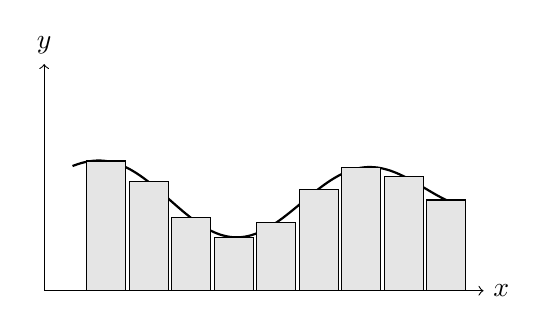
\begin{tikzpicture}[scale=0.9]
  \draw[->] (0,0)--(6.2,0) node[right] {$x$};
  \draw[->] (0,0)--(0,3.2) node[above] {$y$};
  \draw[thick,smooth,domain=0.4:5.8,samples=80] plot(\x,{1.2+0.45*sin(100*\x)+0.04*(\x-3)^2});
  \foreach \x in {0.6,1.2,...,5.4}{
    \draw[fill=gray!20] (\x,0) rectangle +(0.55,{1.2+0.45*sin(100*(\x+0.27))+0.04*(\x+0.27-3)^2});
  }
\end{tikzpicture}
\caption{A schematic midpoint Riemann sum.  The exact picture is less important than the limiting idea.}
\end{figure}

\section{Complex Riemann sums}

For a complex path \(K\), divide the path into small directed pieces \(\Delta_i\).  Choose sample points \(z_i\) on the path.  The complex Riemann sum is
\[
  \sum_i f(z_i)\Delta_i.
\]
Each term means: take the tiny tangent displacement \(\Delta_i\), multiply it by the complex number \(f(z_i)\), thereby scaling and rotating it, and then add all these transformed displacements.

This gives the geometric meaning of
\[
  \int_K f(z)\,dz.
\]
A complex integral is not area in the usual sense.  It is a limit of transformed tangent vectors.

\section{Integrals of powers on the unit circle}

The note states the key example:
\[
  \gamma(t)=e^{it},\qquad 0\le t\le2\pi.
\]
Then
\[
  \int_\gamma z^m\,dz
  =
  \int_0^{2\pi} e^{imt}ie^{it}\,dt
  =
  i\int_0^{2\pi} e^{i(m+1)t}\,dt.
\]
If \(m\neq-1\), then the exponential completes full oscillations and cancels out:
\[
  \int_\gamma z^m\,dz=0.
\]
If \(m=-1\), then the integrand is simply \(i\), so
\[
  \int_\gamma \frac1z\,dz=2\pi i.
\]
Thus
\[
  \int_\gamma z^m\,dz=
  \begin{cases}
  2\pi i,&m=-1,\\
  0,&m\neq-1.
  \end{cases}
\]
This is the seed of residue theory.  The function \(1/z\) is special because it detects the winding of the loop around the origin.

\section{Cauchy--Goursat theorem}

The last page states the Cauchy--Goursat theorem: if \(f\) is holomorphic on a simply connected domain \(\Omega\), then for every closed contour \(\gamma\) in \(\Omega\),
\[
  \int_\gamma f(z)\,dz=0.
\]
The note compares two paths with the same endpoints and suggests path independence in simply connected domains.  This is the right intuition.  If every loop can contract without crossing a singularity, holomorphic integrals do not accumulate circulation.


\section{Contour integrals depend on paths}

For a complex function, the integral
\[
  \int_\gamma f(z)\,dz
\]
depends on both the function and the path \(\gamma\).  A parametrization \(z=\gamma(t)\) gives
\[
  \int_\gamma f(z)\,dz=\int_a^b f(\gamma(t))\gamma'(t)\,dt.
\]
Thus complex integration is line integration in the plane with complex multiplication built in.

\section{Primitive functions and path independence}

If \(f=F'\) on a domain, then
\[
  \int_\gamma f(z)\,dz=F(\gamma(b))-F(\gamma(a)).
\]
So integrals over closed curves vanish.  Conversely, on nice domains, vanishing around closed curves is closely related to the existence of a primitive.  This is the beginning of Cauchy's theorem.

\section{Why singularities matter}

The function \(1/z\) has no primitive on \(\mathbb C\setminus\{0\}\).  Around the unit circle,
\[
  \int_{|z|=1}\frac1z\,dz=2\pi i.
\]
The nonzero integral detects the hole at the origin.  This is the geometric heart of residue theory.

\section{Expanded synthesis and advanced context}

The important insight is that complex integration is simultaneously analytic and topological.  Analytic regularity says holomorphic functions have local antiderivative-like behavior.  Topology says singularities and holes can obstruct cancellation.  The integral of \(1/z\) around the unit circle is the prototype: the local function looks harmless away from \(0\), but the loop winds around a missing point and records \(2\pi i\).


\paragraph{Expanded synthesis.}
For this chapter, the elementary material should be read as a study of why complex integration depends on paths, singularities, and holomorphic structure. The earlier sections compare real and complex integrals, introduce contours and parametrization, and reinterpret Riemann sums in the complex plane.

The deeper object is not a matrix but a differential form on a domain.  The central question is whether its integral depends only on endpoints or also on the chosen path.

The structural hierarchy is as follows. Kernels record what a map forgets, images record what it reaches, cokernels record obstructions to solvability, and quotients record information after an equivalence has been imposed. Determinants act on the top exterior power and therefore measure oriented volume; traces are invariant under cyclic rearrangement and become characters in representation theory; adjoints depend on an inner product and lead to self-adjoint spectral theory.

A useful way to return to the computations is to ask, for every formula, which invariant it is measuring. Row reduction measures rank and kernel; diagonalization measures decomposition into invariant subspaces; Gram--Schmidt measures orthogonal projection; positive definiteness measures ellipsoid geometry; tensor notation measures how components transform. The elementary methods are therefore the finite-dimensional laboratory in which duality, quotienting, functoriality, and spectral decomposition can be seen clearly.
